


\subsection{Architecture}


\subsubsection{ReactJS \& Project Structure}
\begin{figure}[!htbp]
\centering
\begin{forest}
  for tree={
    font=\ttfamily,
    grow'=0,
    child anchor=west,
    parent anchor=south,
    anchor=west,
    calign=first,
    edge path={
      \noexpand\path [draw, \forestoption{edge}]
      (!u.south west) +(7.5pt,0) |- node[fill,inner sep=1.25pt] {} (.child anchor)\forestoption{edge label};
    },
    before typesetting nodes={
      if n=1
        {insert before={[,phantom]}}
        {}
    },
    fit=band,
    before computing xy={l=15pt},
  }
[client
  [components/
    [AppBar/
      [index.js]
      [style.css]
    ]
    [...]
  ]
  [containers/]
  [models/]
  [utils/]
  [index.js]
  [index.html]
  [...]
]
\end{forest}
\caption{Overview of server app's file structure}
\label{fig:server-file-structure-imp}
\end{figure}



\subsubsection{Achitecture of Client}

\begin{figure}[!htbp]
  \centering
    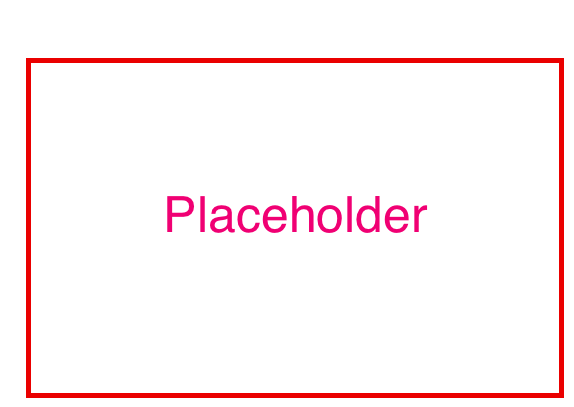
\includegraphics[width=0.6\textwidth]{Figures/placeholder.png}
  \caption{Overview of client architecture}
  \label{fig:client-arch-imp}
\end{figure}
% client arch, App -> router -> container -> components(Compisition... for containers!)

\begin{lstlisting}[language=HTML, caption=Router in client app , label={list:router-client-imp}]
<Router history={history}>
  <Route path="/" component={App}>
    <Route path="auth" component={AuthView} >
      <Route path="login" component={AuthView} />
      <Route path="signup" component={AuthView} />
    </Route>
    <Route component={IndexPage}>
      <Route path="courses" component={CoursesView} />
    </Route>
    <Route path="courses/:courseId" component={QuestionsPage} />
    <Route path="questions/:questionId" component={AnswersPage} />
  </Route>
</Router>
\end{lstlisting}





\subsection{React Containers \& Components}


\subsection{Data Flow}

\subsubsection{Flux Architecture}

\subsubsection{Data Fetching}
